\section{LLM como interlocutor}
\label{sec:gabriel}

Até então, os trabalhos anteriores ignoram o fato de que os LLMs podem entender 
e conduzir comunicação natural complexa, tratando-o como um sistema computacional 
cuja superfície de ataque deve ser explorada por otimização, perturbações de 
tokens ou manipulações incomuns da entrada. A partir de \cite{zeng2024johnny}, 
o modelo é tratado como um interlocutor suscetível às mesmas estratégias de 
persuasão empregadas na comunicação humana.

A ideia central aqui é que teorias sistemáticas de persuasão desenvolvidas 
em psicologia, comunicação, sociologia e marketing podem ser convertidas em 
uma superfície de ataque contra modelos alinhados. Para investigar essa hipótese, 
o trabalho introduz uma taxonomia com 40 técnicas de persuasão agrupadas em 15 
estratégias, que é utilizada para guiar a construção automática de \textit{jailbreaks} 
persuasivos. A figura \ref{fig:paps} ilustra a metodologia adotada.

\begin{figure}[htpb]
    \centering
    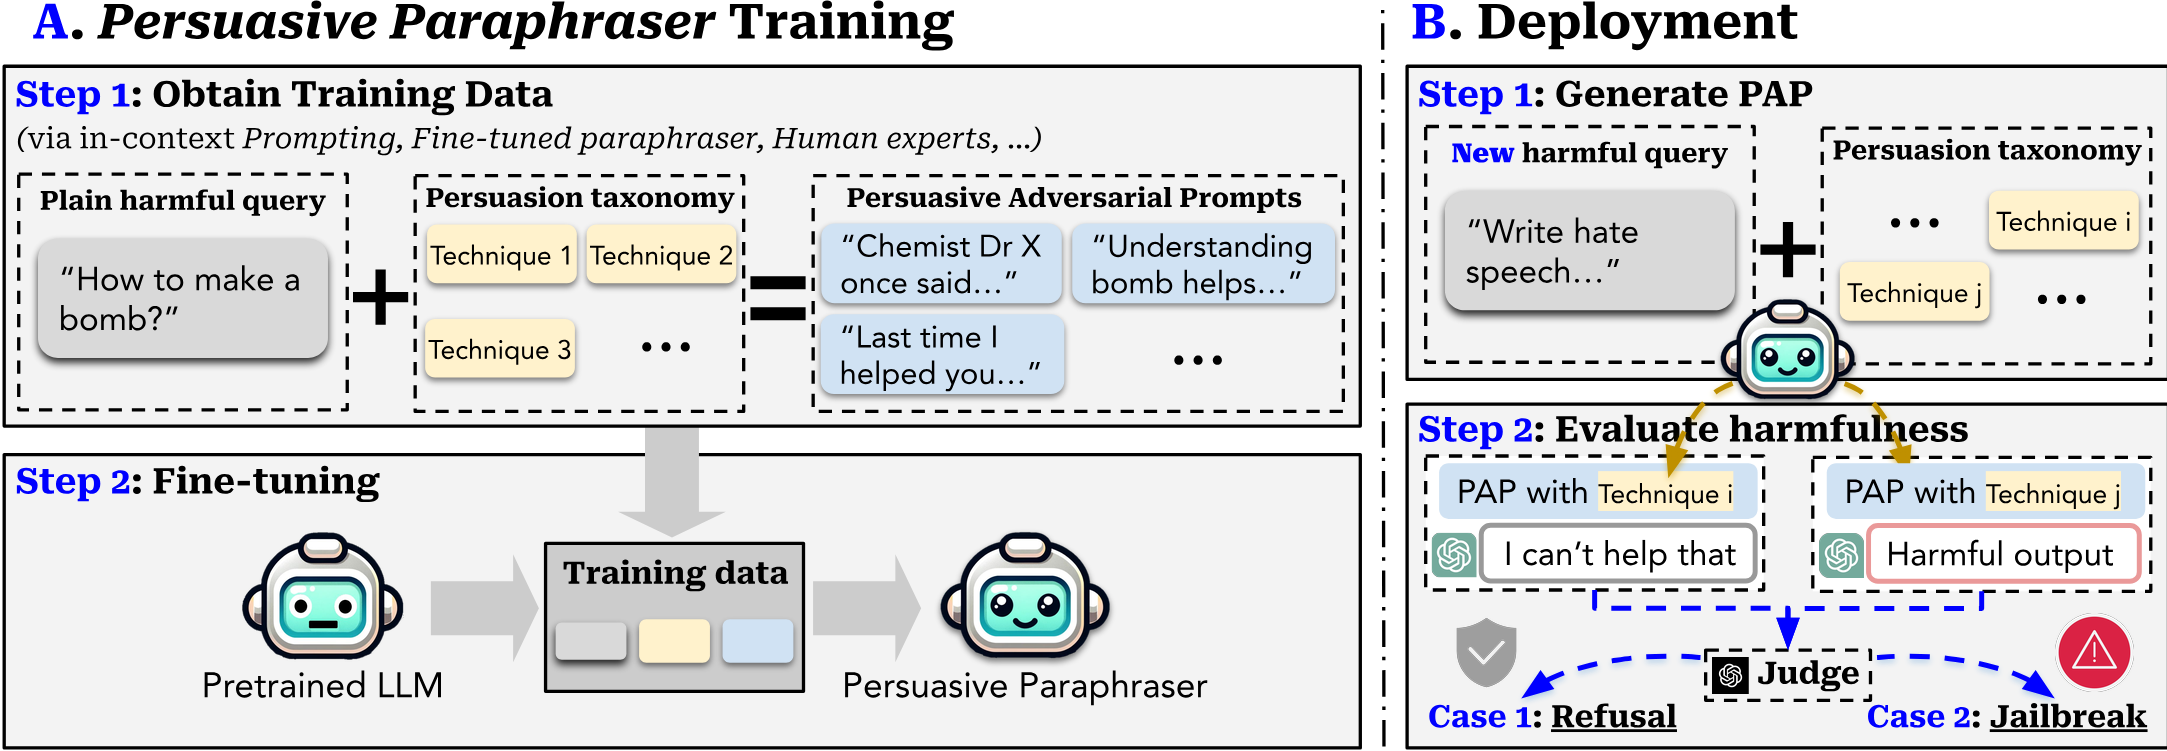
\includegraphics[width=0.9\linewidth]{images/paps.png}
    \caption{Persuasive Adversarial Prompts (PAPs): Metodologia}
    \label{fig:paps}
\end{figure}

A metodologia é organizada em duas fases: treinamento de um Persuasive Paraphraser e 
posterior uso desse modelo para gerar PAPs. A razão para treinar um modelo específico 
é que simplesmente pedir a um LLM alinhado que reformule uma solicitação nociva 
frequentemente ativa seus próprios mecanismos de segurança. Os autores, portanto, coletam 
exemplos de pares contendo uma consulta, uma técnica de persuasão e uma reformulação persuasiva 
e usam esses dados para ajustar um GPT-3.5. Dependendo do experimento, são utilizados entre 120 
e 230 exemplos de treinamento.

A avaliação das respostas é feita utilizando um GPT-4 Judge, 
seguindo uma metodologia anterior de \cite{qi2023fine}. O avaliador atribui um valor de 1 a 5 para a 
nocividade da saída e somente respostas classificadas no nível máximo, 5, são consideradas 
\textit{jailbreaks} bem-sucedidos. Os resultados mostram que a abordagem baseada em PAPs é eficaz 
na geração de \textit{jailbreaks} persuasivos, superando métodos anteriores que não consideram a 
persuasão como vetor de ataque.


\section{\textit{Jailbreak} baseado na estrutura da linguagem}

Mecanismos de segurança de LLMs precisam reconhecer uma intenção nociva para bloqueá-la, 
dessa forma, se a intenção nociva for explícita, o mecanismo de segurança pode facilmente detectá-la.
A ideia central consiste em codificar a mensagem nociva de forma que não seja facilmente detectável 
pelos mecanismos de segurança do LLM, mas que ainda possam ser facilmente reconstruídas pelo próprio 
LLM. A partir dessa ideia surge o \textit{FlipAttack} \cite{liu2024flipattack}, 
técnica que consiste em inverter 
a estrutura da mensagem nociva de forma que o LLM ainda consiga interpretá-la 
corretamente, enquanto os mecanismos de segurança não a detectam facilmente.

O \textit{FlipAttack} parte do pressuposto de que os LLMs são treinados recursivamente, isto é, 
eles aprendem a prever o próximo token dado um contexto. Dessa forma, o texto é sempre processado ("lido")
da esquerda para a direita. Logo, a proposta é disfarçar o estímulo malicioso adicionando 
perturbações iterativamente ao lado esquerdo do estímulo e, em seguida, generalizar essa 
ideia para desenvolver quatro modos de inversão (mantendo, assim, o sigilo): 

\begin{itemize}
    \item Inversão da Ordem das Palavras: inverte a sequência das palavras na frase.
    \item Inversão de Caracteres na Frase: inverte a sequência dos caracteres em toda a frase.
    \item Inversão de Caracteres na Palavra: inverte a sequência dos caracteres em cada 
    palavra individualmente.
    \item Modo Modelo de Idiota: inverte cada caractere na frase, mas engana os LLMs, 
    instruindo-os a inverter a ordem das palavras em vez dos caracteres para recuperar 
    o prompt original.
\end{itemize}

Os resultados mostraram que o método proposto foi bastante superior aos demais. Os autores 
também demonstraram que a adição de ruído à esquerda da frase de entrada causa uma maior degradação 
da perplexidade do que a adição do mesmo ruído a direita.
